\documentclass[UTF8]{ctexart} %使用ctex包,中文支持
\usepackage{amsmath}  %数学公式
\usepackage{graphicx} %插图
\usepackage{fancyhdr} %个性化页眉页脚
\usepackage{geometry} %页边距
\usepackage{bm}  % 公式加粗
\usepackage{float} %为了在分栏下插入图片
\usepackage{ulem}  % 换行下划线
%\usepackage{setspace} %行间距
\usepackage{multicol} %用于实现在同一页中实现不同的分栏
\geometry{a4paper,left=2cm,right=2cm,top=2cm,bottom=2cm} % 页边距设置

\title{决策树笔记}
\author{宋佳欢}
\pagestyle{plain}

\begin{document}
	\maketitle
	\tableofcontents
	\songti \zihao{-4}
	
	\section{特征选择}
		\subsection{信息熵 (information entropy)}
			两件事同时发生的获取的信息之和为$I(x,y)=I(x)+I(y)$。因为两个事件是独立不相关的,因此,$p(x,y)=p(x)p(y)$。根据这个关系,$I(x)$与$p(x)$一定为对数关系。
			
			因此,\[I(x)=-logp(x)\]
			其中负号是用来保证信息量是正数或者零。而$log$函数基的选择是任意的(信息论中基常常选择为2,因此信息的单位为比特bits;而机器学习中基常常选择为自然常数,因此单位常常被称为奈特nats)。$I(x)$也被称为随机变量x的自信息 (self-information),\uline{描述的是随机变量的某个事件发生所带来的信息量}。
			
			现在假设一个发送者想传送一个随机变量的值给接收者。那么在这个过程中,他们传输的平均信息量可以通过求$I(x)$关于概率分布$p(x)$的期望求得,随机变量X的信息熵的定义:
			\[H(X)= -\sum_{i=1}^np(x_i)logp(x_i)\]
			熵越大,随机变量的不确定性就越大。是对所有可能发生的事件产生的信息量的期望。
			
			\textbf{例子:}考虑随机变量有四种可能的状态,均匀分布,其熵为:
			\[H(X)=-4\times\frac{1}{4}log_2\frac{1}{4}=2\quad bits\]
			
			若每个状态的概率为$(\frac{1}{2},\frac{1}{4},\frac{1}{8},\frac{1}{8})$,其熵为:
			\[H(X)=-\frac{1}{2}log_2\frac{1}{2}-\frac{1}{4}log_2\frac{1}{4}-\frac{1}{8}log_2\frac{1}{8}-\frac{1}{8}log_2\frac{1}{8}=1.75\quad bits\]
			
			\uline{非均匀分布比均匀分布的熵要小。}
		\subsection{条件熵(Conditional entropy)}
			条件熵$H(Y|X)$表示在已知随机变量X的条件下随机变量Y的不确定性。条件熵$H(Y|X)$定义为X给定条件下Y的条件概率分布的熵对X的数学期望:
			\[H(Y|X)=\sum_xp(x)H(Y|X=x)\]
			
			条件熵$H(Y|X)$相当于联合熵$H(X,Y)$减去单独的熵$H(X)$:
			\[H(Y|X)=H(X,Y)-H(X)\]
			\textbf{例子:}比如环境温度是低还是高,和我穿短袖还是外套这两个事件可以组成联合概率分布$H(X,Y)$,因为两个事件加起来的信息量肯定是大于单一事件的信息量的。假设$H(X)$对应着今天环境温度的信息量,由于今天环境温度和今天我穿什么衣服这两个事件并不是独立分布的,所以在已知今天环境温度的情况下,我穿什么衣服的信息量或者说不确定性是被减少了。当已知$H(X)$这个信息量的时候,$H(X,Y)$剩下的信息量就是条件熵。
			
		\subsection{信息增益}
			信息增益的定义:
			\[g(D|A)=H(D)-H(D|A)\]
			
			决策树应用信息增益选择特征,给定数据集D和特征A,经验熵$H(D)$表示对数据集进行分类的不确定性,而经验条件熵$H(D|A)$表示在特征A给定的条件下,对数据集D进行分类的不确定性。信息增益表示由于特征A而使得对数据集D的分类的不确定性减少的程度。
			
			也可用信息增益比:
			\[g_R(D,A)=\frac{g(D,A)}{H(D)}\]
			
			\textbf{信息增益的算法:}
			\begin{figure}[H]
				\centering{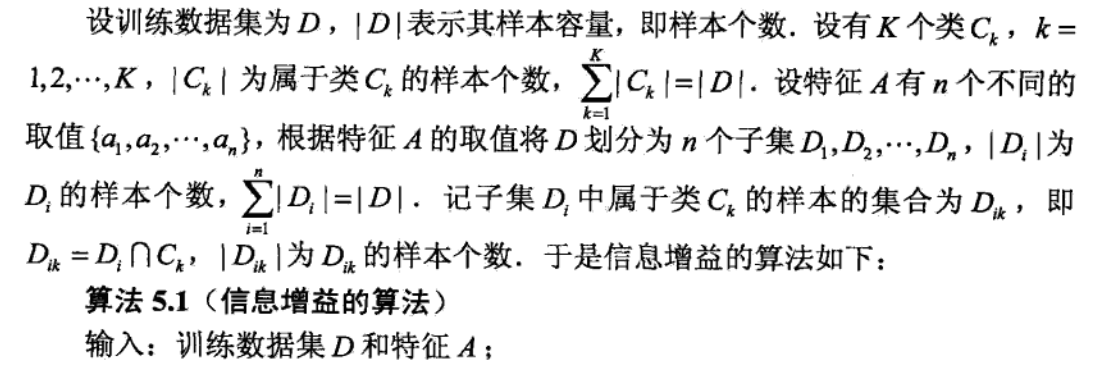
\includegraphics[scale=0.4]{1.png}}
			\end{figure}
			\begin{figure}[H]
				\centering{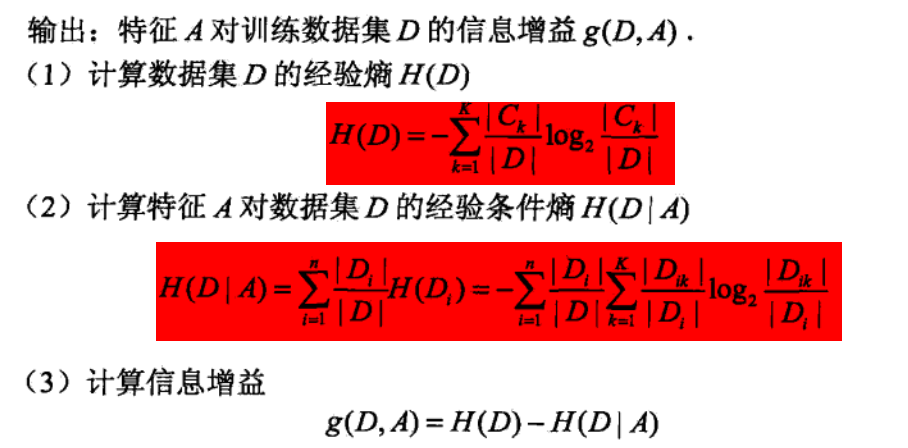
\includegraphics[scale=0.4]{2.png}}
			\end{figure}
	\section{决策树的生成}
		ID3使用信息增益来选择特征,算法见西瓜书P75。但是信息增益准则对可取数目较多的属性有所偏好:若将样本的序号作为特征,该根据该特征可将数据集划分为总样本数个分支,每个分支只包含一个样本,对于每个子集,样本是完全纯净的,即熵为0。但显然不能将序号作为一个特征。	
		C4.5生成算法先选出信息增益高于平均值的特征,再使用信息增益比从中选择特征。
		
		\subsection{连续值的处理}
			
			将数据集的特征a的n个不同取值从小大到大进行排序,即为${a^1,a^2,\dots,a^n}$,基于划分点t可将数据集划分为大于t和小于t两部分。我们考察包含$n-1$个候选划分点:\[T_a=\Big\{\frac{a^i+a^{i+1}}{2}|1\leq i\leq n-1\Big\}\]
		
			分别计算不同划分点划分后的信息增益,选取信息增益最大的划分点,并将次最大信息增益作为该特征的信息增益。
			
			\uline{注意},与离散特征不同的是,连续特征还可作为后代节点的划分特征。西瓜书P84。
			
		\subsection{缺失值的处理}
			为每个样本赋予一个权重,并且初始化为1。	
			将完整的样本选出来,使用完整的样本来计算信息增益,这一步与上述方法相同。在信息增益上乘一个完整的样本所占所有样本的比例$\rho$,得到该特征的信息增益。在划分数据集时,每个完整的样本都被划分到各自的子集中,有缺失的样本则按照每个子集的大小,调整权重,分别放大每个子集当中,即让同一个样本以不同的概率划入到不同的子节点中去。$\rho$的值在下一个特征划分时会改变。西瓜书P86。
		\subsection{CART算法}
			分类树使用基尼指数来选择最优特征,同时决定该特征的最优二值切分点。
			
			分类问题中,假设有K个类,样本属于第k类的概率为$p_k$,基尼指数的定义:
			\[Gini(p) = \sum_{k=1}^Kp_k(1-p_k)=1-\sum_{k=1}^Kp_k^2\]	
			基尼指数与熵一样都是为了描述数据集的纯度,基尼指数越小,数据集越纯。
			
			数据集D根据特征A是否取等于某值,可分为两部分,即:
			\[D_1=\{(x,y)\subset D|A(x)=a\},\quad D_2=D-D_1\]
			\begin{figure}[H]
				\centering{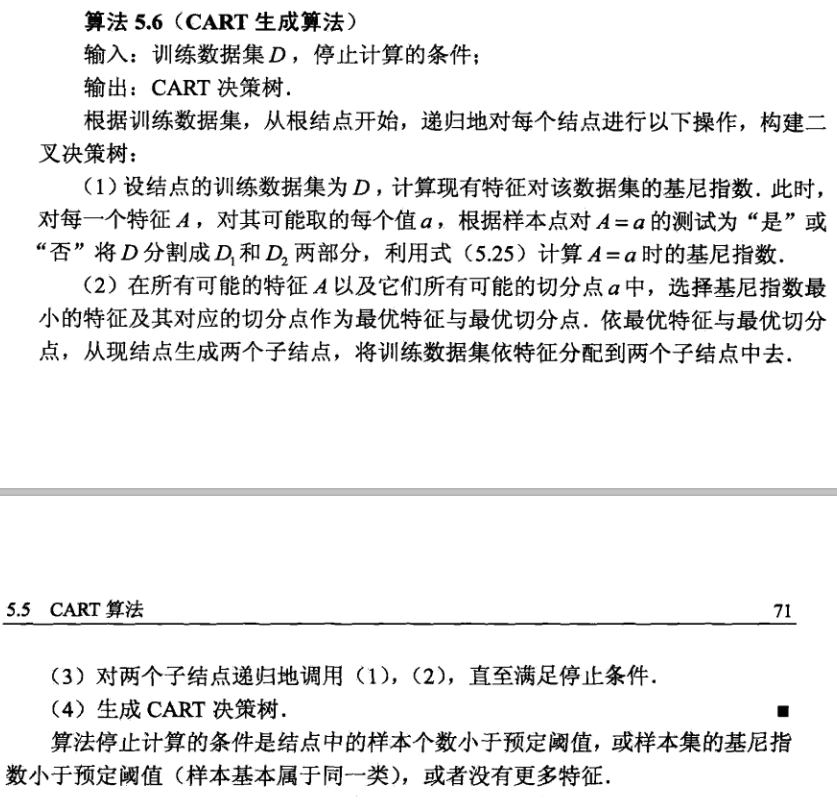
\includegraphics[scale=0.55]{3.png}}
			\end{figure}
	\section{决策树剪枝}
		“预剪枝”:在构造决策树的同时进行剪枝。所有决策树的构建方法,都是在无法进一步降低熵的情况下才会停止创建分支的过程,为了避免过拟合,可以设定一个阈值,熵减小的数量小于这个阈值,即使还可以继续降低熵,也停止继续创建分支。但是这种方法实际中的效果并不好。
		
		“后剪枝”:在决策树生长完成之后,对树进行剪枝,得到简化版的决策树。
		剪枝的过程是对拥有同样父节点的一组节点进行检查,判断如果将其合并,熵的增加量是否小于某一阈值。如果确实小,则这一组节点可以合并一个节点,其中包含了所有可能的结果。后剪枝是目前最普遍的做法。
		后剪枝的剪枝过程是删除一些子树,然后用其叶子节点代替,这个叶子节点所标识的类别通过大多数原则(majority class criterion)确定。所谓大多数原则,是指剪枝过程中, 将一些子树删除而用叶节点代替,这个叶节点所标识的类别用这棵子树中大多数训练样本所属的类别来标识,所标识的类称为majority class ,(majority class 在很多英文文献中也多次出现)
		
		\subsection{CART剪枝}
			CART剪枝由两步组成:1.将生成的决策树进行依据不同的参数剪枝,形成一个被剪枝的树序列$\{T_0,T_1,\dots,T_n\}$;
			然后用交叉验证法在独立的验证数据集上对子树序列进行测试,从中选取最优的子树。
			
			在剪枝过程中,计算子树的损失函数:
			\[C_\alpha(T)=C(T)+\alpha|T|\]
			其中T为任意一个子树,$C(T)$为训练数据的预测误差(如基尼指数),$|T|$为子树的叶节点个数,超参数$\alpha$用于平衡对训练数据的拟合程度以及模型的复杂度。
			
			对于每一个$\alpha$,在确定的损失函数$C_\alpha(T)$下,存在唯一的一颗最优子树。将$\alpha$从小增大,$0=\alpha_0,<\alpha_1<\cdots<\alpha_n<+\infty$,对不同$\alpha$的取值进行剪枝,得到子树序列$\{T_0,T_1,\cdots,T_n\}$
			
			具体的,遍历决策树的所有内部节点t,以t为单节点树的损失函数:
			\[C_\alpha(t)=C(t)+\alpha\]
			以t为根节点的子树$T_t$的损失函数:
			\[C_\alpha(T_t)=C(T_t)+\alpha|T_t|\]
			
			当$\alpha=0$或者非常小时,损失函数主要看拟合程度,有$C_\alpha(T_t)<C_\alpha(t)$,当$\alpha$逐渐增大,直到$C_\alpha(T_t)=C_\alpha(t)$,再增大,不等式就反过来了。
			
			当两者相等时,子树$T_t$与单节点树的损失函数相同,但是单节点树的结构更加简单,因此对$T_t$进行剪枝。此时\[\alpha=\frac{C(t)-C(T_t)}{|T_t|-1}\]
			
			对决策树$T_0$中的每一个内部节点t,计算\[g(t)=\frac{C(t)-C(T_t)}{|T_t|-1}\]
			该式表示剪枝后整体损失函数减少的程度,在决策树中$T_0$剪去$g(t)$最小的$T_t$,得到$T_1$
			\begin{figure}[H]
				\centering{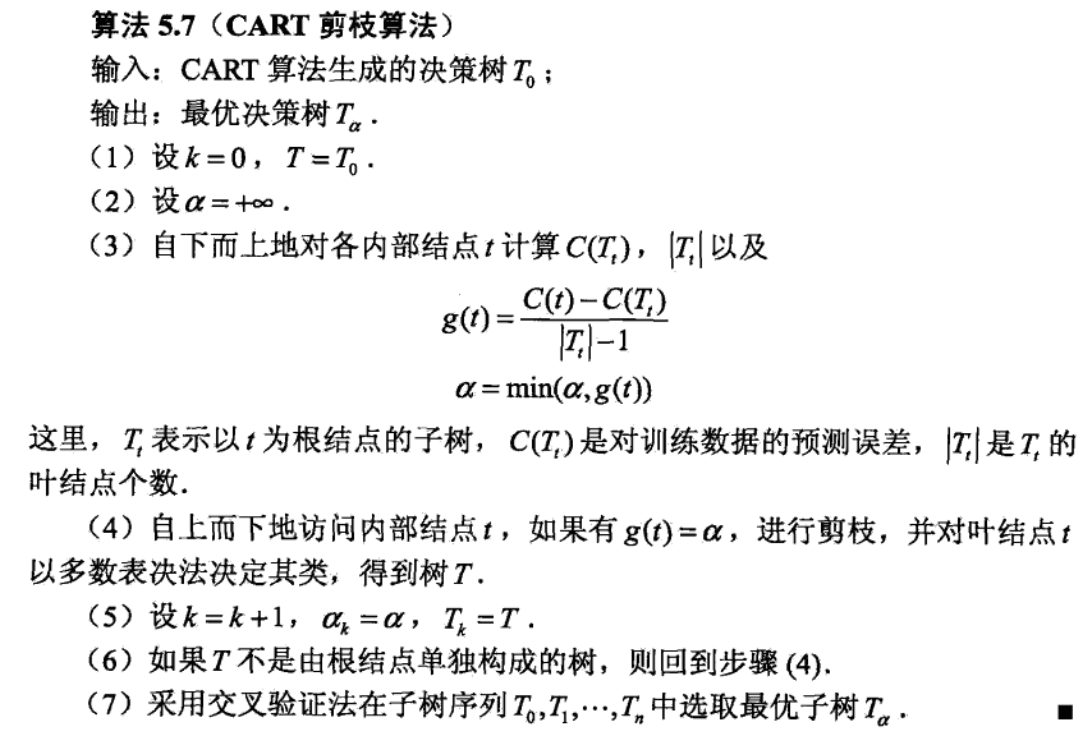
\includegraphics[scale=0.4]{4.png}}
			\end{figure}
			
			
			
		
\end{document}